\documentclass[tikz,border=8pt]{standalone}
% Shared look for every TikZ diagram. Load with \input{../../tools/tikz-style.tex}
\usepackage[T1]{fontenc}
\usepackage{lmodern}
\renewcommand{\sfdefault}{lmr}  % diagrams use the same serif as the text
\usetikzlibrary{arrows.meta, positioning, shapes.geometric, calc, fit, backgrounds}
\definecolor{cblue}{HTML}{4C78A8}
\definecolor{corange}{HTML}{F58518}
\definecolor{cgreen}{HTML}{54A24B}
\definecolor{cred}{HTML}{E45756}
\definecolor{cpurple}{HTML}{B279A2}
\definecolor{cgrey}{HTML}{6B6B6B}
\tikzset{
  every picture/.style={font=\sffamily, line width=1.2pt},
  box/.style={draw=#1, fill=#1!12, rounded corners=4pt, align=center, inner sep=7pt, minimum height=1.1cm},
  box/.default=cgrey,
  arrow/.style={-{Stealth[length=3mm]}, draw=cgrey, line width=1.4pt},
  title/.style={font=\sffamily\bfseries\Large},
  note/.style={font=\sffamily\small, text=cgrey, align=center},
}
\AtBeginDocument{\hyphenpenalty=10000 \exhyphenpenalty=10000}

% Without gamma: from a given start, each end position is reached by exactly one circular arc that leaves along the
% start heading, so the end heading is fixed by the end position (end heading = 2 x chord angle - start heading). With gamma, the end heading can differ.
\begin{document}
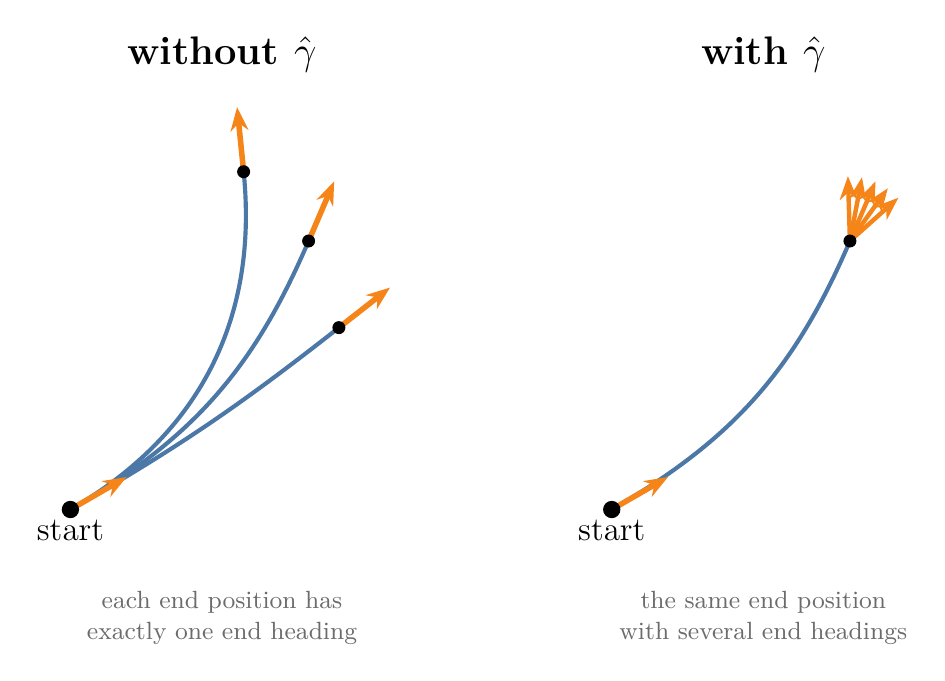
\begin{tikzpicture}[scale=5.5, every node/.append style={font=\large}]
  \begin{scope}
    \node[title] at (0.35,1.05) {without $\hat\gamma$};
    \foreach \ex/\ey/\ang in {0.55/0.62/66.8, 0.62/0.42/38.1, 0.4/0.78/95.8} {
      \draw[cblue, line width=1.5pt] (0,0) to[out=30, in=\ang+180] (\ex,\ey);
      \draw[-{Stealth[length=3mm]}, corange, line width=2pt] (\ex,\ey) -- ++(\ang:0.15);
      \fill[black] (\ex,\ey) circle (0.015);
    }
    \draw[-{Stealth[length=3mm]}, corange, line width=2pt] (0,0) -- (30:0.15);
    \fill[black] (0,0) circle (0.02) node[below] {start};
    \node[note, align=center] at (0.35,-0.25) {each end position has\\exactly one end heading};
  \end{scope}
  \begin{scope}[xshift=1.25cm]
    \node[title] at (0.35,1.05) {with $\hat\gamma$};
    \draw[cblue, line width=1.5pt] (0,0) to[out=30, in=246.8] (0.55,0.62);
    \foreach \ang in {41.8,54.3,66.8,79.3,91.8} \draw[-{Stealth[length=3mm]}, corange, line width=1.6pt] (0.55,0.62) -- ++(\ang:0.15);
    \fill[black] (0.55,0.62) circle (0.015);
    \draw[-{Stealth[length=3mm]}, corange, line width=2pt] (0,0) -- (30:0.15);
    \fill[black] (0,0) circle (0.02) node[below] {start};
    \node[note, align=center] at (0.35,-0.25) {the same end position\\with several end headings};
  \end{scope}
\end{tikzpicture}
\end{document}
